\section{Εισαγωγή}

Τα συστήματα αυτοματισμού είναι πλέον μέρος της καθημερινότητας μας. Συναντάμε συνέχεια, χωρίς
απαραίτητα να το συνειδητοποιούμε κάποιου είδος σύστημα το οποίο είναι προγραμματισμένο να εκτελεί
μια διεργασία με βάση ορισμένες συνθήκες του εξωτερικού του περιβάλλοντος. Το παραπάνω έχει μεγάλο
αντίκτυπο στον κόσμο το οποίο γίνεται ξεκάθαρο με την ραγδαία εξέλιξη του IoT (Internet of Things).
Περιτριγυριζόμαστε από συσκευές οι οποίες λειτουργούν ως συστήματα αυτοματισμού αλλά παράλληλα
επικοινωνούν με το Cloud. Από την πλευρά των προγραμματιστών προσφέρονται άπειρες συσκευές με τις
δικές τους ιδιαιτερότητες και άπειρα εργαλεία που λειτουργούν στην κάθε συσκευή.
Δεν είναι όμως ξεκάθαρο το πιο είναι καλύτερο για κάθε use-case. Στην εκάστοτε
εργασία θα χρησιμοποιήσουμε τον μικροελεγκτή ESP32C6-DevKitC-1 και θα γίνει μια απόπειρα
σύγκρισης τριών διαφορετικών οικοσυστημάτων προγραμματισμού (Arduino, Rust-Embassy, ESP-IDF).
Με σκοπό την πλήρης διαφάνεια των αποτελεσμάτων το παρακάτω κεφάλαιο εξηγεί την απαραίτητη
θεωρία για την κατανόηση των συστημάτων αυτοματισμού, του μικροελεγκτή και τα KPI (Key
Perfomance Indicators) που θα μετρήσουμε.

\subsection{Συστήματα Αυτοματισμού}

\begin{figure}[h!]
\centering
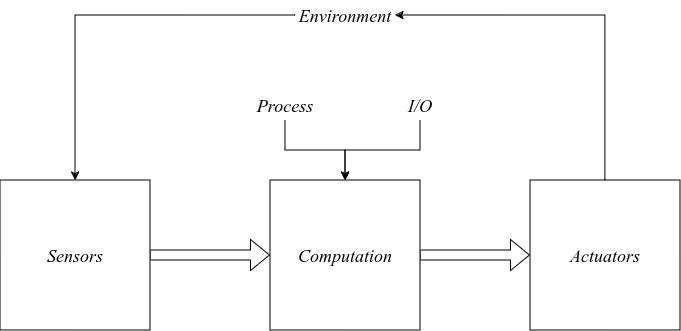
\includegraphics[scale=0.4]{images/introduction/as_elements.png}
\caption{Αναπαράσταση βασικών στοιχείων συστημάτων αυτοματισμού.}
 \label{fig:as_elements}
\end{figure}

Ένα σύστημα αυτοματισμού είναι ένα σύστημα που αποτελείτε από τρία
βασικά στοιχεία:

\begin{enumerate}
\item Τους σένσορες ή αισθητήρες, που λαμβάνουν δεδομένα από το
εξωτερικό τους περιβάλλων και παράγουν ένα όσο το δυνατόν πιο
αξιόπιστο αναλογικό ή ψηφιακό σήμα.
\item Ένα υπολογιστικό σύστημα, για παράδειγμα έναν μικροελεγκτή το
οποίο μπορεί να χρησιμοποιήσει το σήμα των αισθητήρων για
υπολογισμούς, επεξεργασία ή I/O.
\item Το στοιχείο δράσης ή ενεργοποιητής, που με βάση των υπολογισμών
του υπολογιστικού συστήματος ενεργοποιούνται ή παραμένουν
αδρανής. Αυτό το στοιχείο αποτελεί την έξοδο του συστήματος
αυτοματισμού και είναι αυτό το οποίο έχει συνήθως αντίκτυπο στο
εξωτερικό του περιβάλλων.
\end{enumerate}

Το υπολογιστικό σύστημα μπορεί να χρησιμοποιηθεί για να παίρνει
αποφάσεις με βάση των τιμών που δέχεται από τους αισθητήρες και εκεί
φαίνεται η πραγματική χρησιμότητα των αυτόματων συστημάτων. Πολλές
φορές με βάση την λήψη αποφάσεων (υπολογισμών) το αποτέλεσμα του
στοιχείου δράσης χρειάζεται να επιστρέψει στην είσοδο του συστήματος,
για παράδειγμα εάν χρειάζεται να ρυθμιστεί ένας σένσορας δυναμικά. Σε
αυτήν την περίπτωση το σύστημα λέγεται σύστημα ανατροφοδότησης ή
αλλιώς σύστημα κλειστού βρόχου \figref{fig:as_feedback}.

\begin{figure}[h!]
\centering
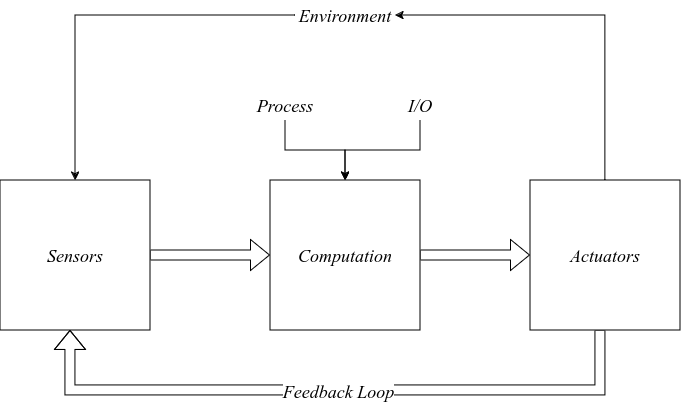
\includegraphics[scale=0.4]{images/introduction/as_feedback.png}
\caption{Σύστημα κλειστού βρόχου.}
 \label{fig:as_feedback}
\end{figure}

Για την παρούσα εργασία μας ενδιαφέρει κυρίως το υπολογιστικό
σύστημα. Συγκεκριμένα, μας ενδιαφέρει ο προγραμματισμός του
μικροελεγκτή ESP32C6, προκύπτει όμως ένα πρόβλημα. Τα συστήματα
αυτοματισμού δεν περιλαμβάνουν την θεωρία προγραμματισμού
μικροελεγκτών, αυτό ισχύει διότι είναι ένα abstraction (αφαίρεση) που
αφαιρεί την ανάγκη συγκεκριμένου υπολογιστικού συστήματος.  Για
παράδειγμα θα μπορούσαμε να χρησιμοποιήσουμε ένα Raspberry Pi, αυτό
δεν θα άλλαζε το γεγονός ότι λειτουργούμε σε ένα σύστημα αυτοματισμού
ασχέτως από το ότι χρησιμοποιούμε ένα single-board computer (SBC) αντί
για ένα micro-controller unit (MCU). Εδώ προκύπτει το ερώτημα, πια η
διαφορά;

\subsection{Embedded Systems}

Ο πιο σύγχρονος τρόπος προγραμματισμού παίρνει μέρος συνήθως σε αυτό
που αποκαλούμε user-space ενός λειτουργικού συστήματος.  Στο
user-space το OS (Operating System) αναλαμβάνει ένα πολύ μεγάλο μέρος
της πολυπλοκότητας του προγραμματισμού. Η δημιουργία εικονικής μνήμης,
η δυνατότητα παράλληλου προγραμματισμού, η διαχείριση μνήμη σορού
(heap memory) είναι όλα προβλήματα που αντιμετωπίζονται σχεδόν
αυτόματα πλέον. Επίσης μέσο του λειτουργικού συστήματος αποκρύβονται
οι λεπτομέρειες του hardware, τα πάντα σχεδόν προσφέρονται ως ψηφιακά
API (Application Programming Interface), τα οποία χτίζονται το ένα
πάνω στο άλλο.  Με κάθε πρόσθεση επιπέδου αφαίρεσης χάνετε λίγο
παραπάνω η ικανότητα πλήρης διαχείρισης του hardware με το θετικό ότι
σε γενικές γραμμές κάνει την ζωή του προγραμματιστή πιο εύκολη. Είναι
ξεκάθαρο λοιπόν ότι τα abstraction layers είναι χρήσιμα, αλλά είναι
δίκοπο μαχαίρι. Από την μια πλευρά η υλοποίηση των περισσότερων
εφαρμογών γίνεται απίστευτα πιο εύκολη. Από την άλλη, τι γίνεται όταν
πραγματικά χρειαζόμαστε να επικοινωνήσουμε με το hardware που έχουμε
μπροστά μας;
Πολλές φορές υπάρχουν συστήματα που δεν μπορούν ή δεν χρειάζεται
να τρέξουν ένα ολόκληρο operating system. Πολλές φορές δεν έχουμε την
επιλογή να τρέξουμε κώδικα πάνω σε ένα abstraction. Για παράδειγμα,
συστήματα που βρίσκονται σε απλές συσκευές όπως θερμοστάτες και
ρολόγια όχι μόνο δεν είναι απαραίτητο να τρέχουν OS αλλά πολλές φορές
δεν είναι βέλτιστο. 
Αναφερόμαστε στα συστήματα που δεν χρησιμοποιούν παραδοσιακά OS  ως
embedded systems διότι τα βρίσκουμε συχνά ενσωματωμένα σε μεγαλύτερες συσκευές.

\begin{figure}[h!]
\centering
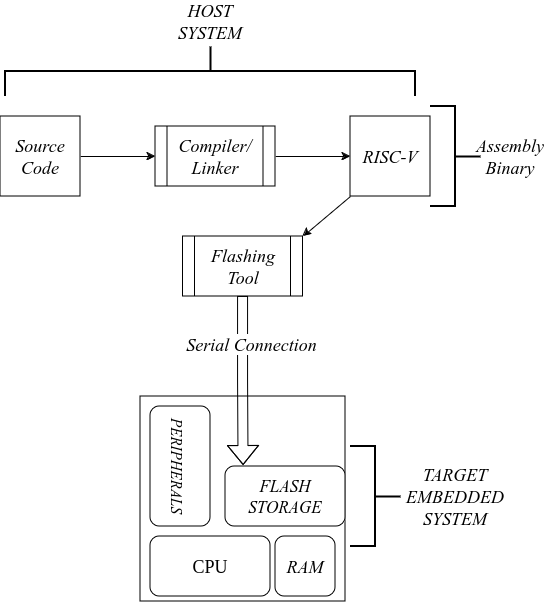
\includegraphics[scale=0.4]{images/introduction/programming_embedded.png}
\caption{Σύστημα κλειστού βρόχου.}
 \label{fig:embedded_workflow}
\end{figure}

Η περίπτωση του ESP32C6 είναι ότι αν και είναι πανίσχυρος για μικροελεγκτής ανάλογα
με το framework περιέχει μινιμαλιστικά, στην καλύτερη περίπτωση, abstractions.

\begin{figure}[!htb]
    \centering
    \begin{minipage}{0.49\textwidth}
        \centering
        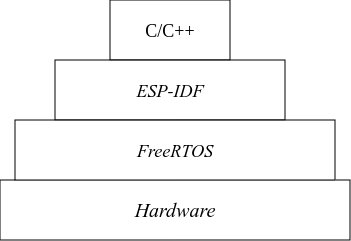
\includegraphics[scale=0.4]{images/introduction/idf_layers}
        \caption{ESP-IDF Abstraction Layers}
        \label{fig:idf_layers}
      \end{minipage}  
    \begin{minipage}{0.49\textwidth}
        \centering
        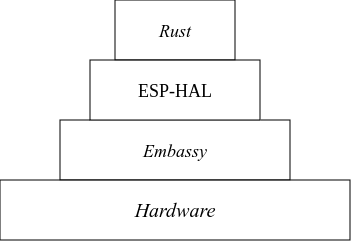
\includegraphics[scale=0.4]{images/introduction/rust_layers}
        \caption{Embassy Abstraction Layers}
        \label{fig:rust_layers}
      \end{minipage}  
    \begin{minipage}{0.49\textwidth}
      \centering
        \vspace{0.5cm}
        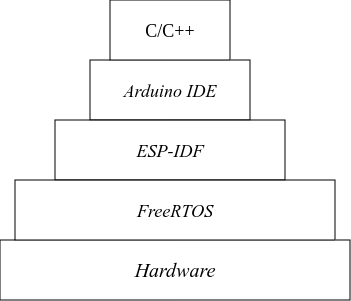
\includegraphics[scale=0.4]{images/introduction/arduino_layers}
        \caption{Arduino Abstraction Layers}
        \label{fig:arduino_layers}
    \end{minipage}%
\end{figure}



